
\documentclass[10pt,a4paper]{article}
\usepackage[dvips]{epsfig}
\usepackage{graphicx}
\oddsidemargin  0 mm
\evensidemargin  0 mm
\voffset -13 mm
\textwidth 160 mm
\textheight 240 mm

\usepackage{fancyhdr}
\pagestyle{fancy}
\lfoot{VA-Tech Hydro, Solver Report}
\rfoot{Eco-Var}

\renewcommand{\headrulewidth}{0.0pt}
\renewcommand{\footrulewidth}{0.4pt}

\begin{document}
\author{VA-Tech Hydro}
\title{Report of HydroSolver}
\date{\today}
\maketitle
{\huge \begin{verbatim}Eco-Var\end{verbatim}}

This is the template version of the hydro report\\
\epsfig{file=MeridCont.eps,width=450\unitlength}
\newpage
{\huge Stage hydraulic data}
\vspace{20pt}\newline
\begin{tabular}{|l|l|l|l|l|l|}
\multicolumn{6}{l}{Stage performance} \\ 
\hline
& Dim & Inlet& IfaStat & IfaRot  & Outlet \\ 
\hline
$\dot m $ & $\frac{kg}{s}$ & 608.863 & 606.001 & 609.412 & 610.104 \\ 
\hline
$\dot q$ & $\frac{m^3}{s}$ & 0.609961 & 0.607093 & 0.610511 & 0.611204 \\ 
\hline
$p_{tot}$ & $Pa$ & 74670 & 73629.7 & 74646.4 & -0.173461 \\ 
\hline
$rc_u$ & $\frac{m^2}{s}$ & 8.72889e-08 & 0.549446 & 0.549791 & 0.0837747 \\ 
\hline
\end{tabular}
\vspace{20pt}\newline
\begin{tabular}{|l|l|l|l|}
\multicolumn{4}{l}{Blade} \\ 
\hline
& & Stator & Rotor\\ 
\hline
$M_z$ &$Nm$ & -333.729& 283.23\\ 
\hline
$\omega$ & $\frac{rad}{s}$ & 0& 154.829\\ 
\hline
\end{tabular}
\vspace{20pt}\newline
\begin{tabular}{|l|l|l|}
\multicolumn{3}{l}{Hydraulic height} \\ 
\hline
$H_{p_{tot}}$ &$\frac{\Delta p^{in,out}_{tot}}{\rho g}$ & 7.62536 \\ 
\hline
$H_{M_z}$ &$\frac{M_z^{Rot} \omega}{g \dot m_{ifa,rot}}$ & 7.33519 \\ 
\hline
$H_{c_u}$ &$\frac{\omega \Delta(r c_u)_{Rot} }{g}$ & 7.35503 \\ 
\hline
\end{tabular}
\vspace{20pt}\newline
\begin{tabular}{|l|l|l|}
\multicolumn{3}{l}{Reference values} \\ 
\hline
$\rho$ &$\frac{kg}{m^3}$ & 998.2 \\ 
\hline
$g$ &$\frac{m}{s^2}$ & 9.81 \\ 
\hline
\multicolumn{3}{|l|}{Reference by Input} \\ 
\hline
$p_{tot,suc}$ &$Pa$ & 0 \\ 
\hline
$\Delta p_{ref}$ &$Pa$ & 108696 \\ 
\hline
$H_{ref}$ &$m$ & 11.1001 \\ 
\hline
\multicolumn{3}{|l|}{$\sigma = press(\sigma) = \frac{p-p_{tot,suc}}{\rho g H_{ref}}$} \\ 
\hline
\end{tabular}
\vspace{20pt}\newline
\begin{tabular}{|l|l|l|}
\multicolumn{3}{l}{Numerical error} \\ 
\hline
$f_{swirl}^{Rot}$ &$1-\frac{H_{M_z}}{H_{c_u}}$ & 0.00269732 \\ 
\hline
$f_{swirl}^{Stat}$ &$1-\frac{{M_z}^{Stat}}{\dot m_{in}\Delta(rc_u)_{Stat}}$ & 0.00241627 \\ 
\hline
$f_{\dot m}^{Stat}$ &$1-\frac{\dot m_{in}}{\dot m_{ifa,stat}}$ & -0.00472292 \\ 
\hline
$f_{\dot m}^{ifa}$ &$1-\frac{\dot m_{ifa,stat}}{\dot m_{ifa,rot}}$ & 0.00559716 \\ 
\hline
$f_{\dot m}^{Rot}$ &$1-\frac{\dot m_{ifa,rot}}{\dot m_{out}}$ & 0.00113487 \\ 
\hline
\end{tabular}
\vspace{20pt}\newline
\begin{tabular}{|l|l|l|}
\multicolumn{3}{l}{Numerical efficiency} \\ 
\hline
$\eta^{Tu}_{num}$ &$\frac{H_{M_z}}{H_{p_{tot,Rot}}}$ & 0.96225 \\ 
\hline
\end{tabular}
\vspace{20pt}\newline
\begin{tabular}{|l|l|l|l|l|}
\multicolumn{5}{l}{Kavitation on rotor blade} \\ 
\hline
$\frac{\Delta A}{A}$ & $0.001$& $0.005$& $0.01$& $0.02$  \\ 
\hline
$p \ [Pa]$ & $-72964.1$& $-64085.5$& $-62459.3$& $-61807.9$  \\ 
\hline
$NPSH_{his}$ & $-7.45113$& $-6.54445$& $-6.37838$& $-6.31186$  \\ 
\hline
$\sigma_{his}$ & $-0.671267$& $-0.589584$& $-0.574624$& $-0.568631$  \\ 
\hline
\end{tabular}
\vspace{20pt}\newline
\begin{tabular}{|l|l|l|}
\multicolumn{3}{l}{Kavitation on rotor hub} \\ 
\hline
$\frac{\Delta A}{A}$ & $0.015$& $0.025$  \\ 
\hline
$p \ [Pa]$ & $-44000.2$& $-42389$  \\ 
\hline
$NPSH_{his}$ & $-4.49333$& $-4.32879$  \\ 
\hline
$\sigma_{his}$ & $-0.404801$& $-0.389978$  \\ 
\hline
\end{tabular}
\vspace{20pt}\newline
\begin{tabular}{|l|l|l|}
\multicolumn{3}{l}{Kavitation on rotor shroud} \\ 
\hline
$\frac{\Delta A}{A}$ & $0.016$& $0.026$  \\ 
\hline
$p \ [Pa]$ & $-52733.6$& $-50558.7$  \\ 
\hline
$NPSH_{his}$ & $-5.38519$& $-5.16308$  \\ 
\hline
$\sigma_{his}$ & $-0.485148$& $-0.465138$  \\ 
\hline
\end{tabular}

\newpage
{\huge Kc} \\
Remark: $kcm = \sqrt{kcr^2+kcax^2}$\\
Inlet: \\
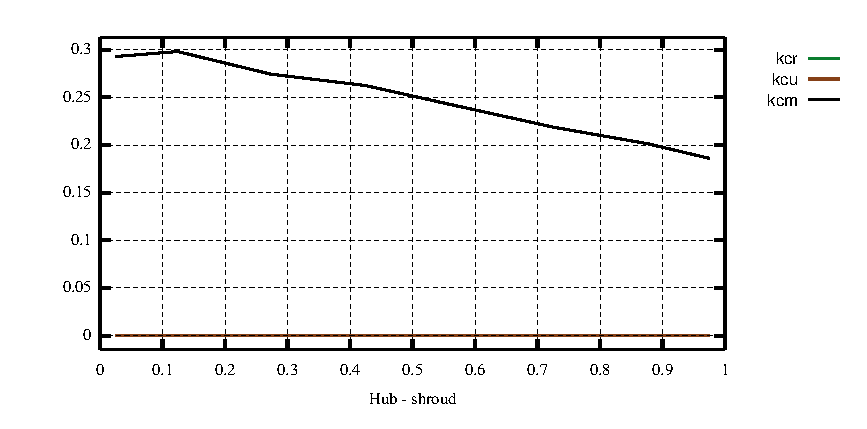
\epsfig{file=InletKC.eps,width=400\unitlength}\\
Interface: \\
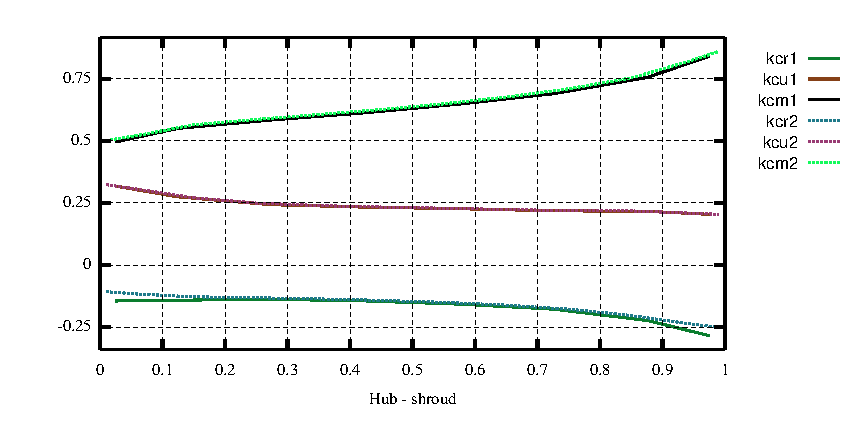
\epsfig{file=InterfaceKC.eps,width=400\unitlength}\\
Outlet: \\
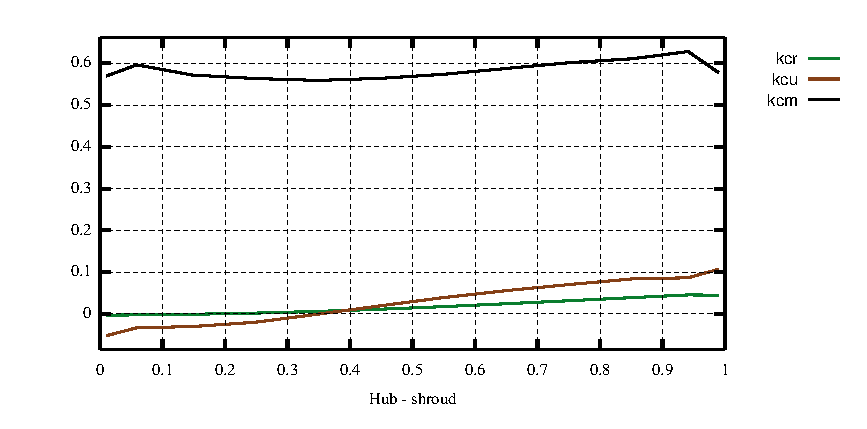
\epsfig{file=OutletKC.eps,width=400\unitlength}\\
\newpage
{\huge All overview}\\ press ($\sigma$) \\
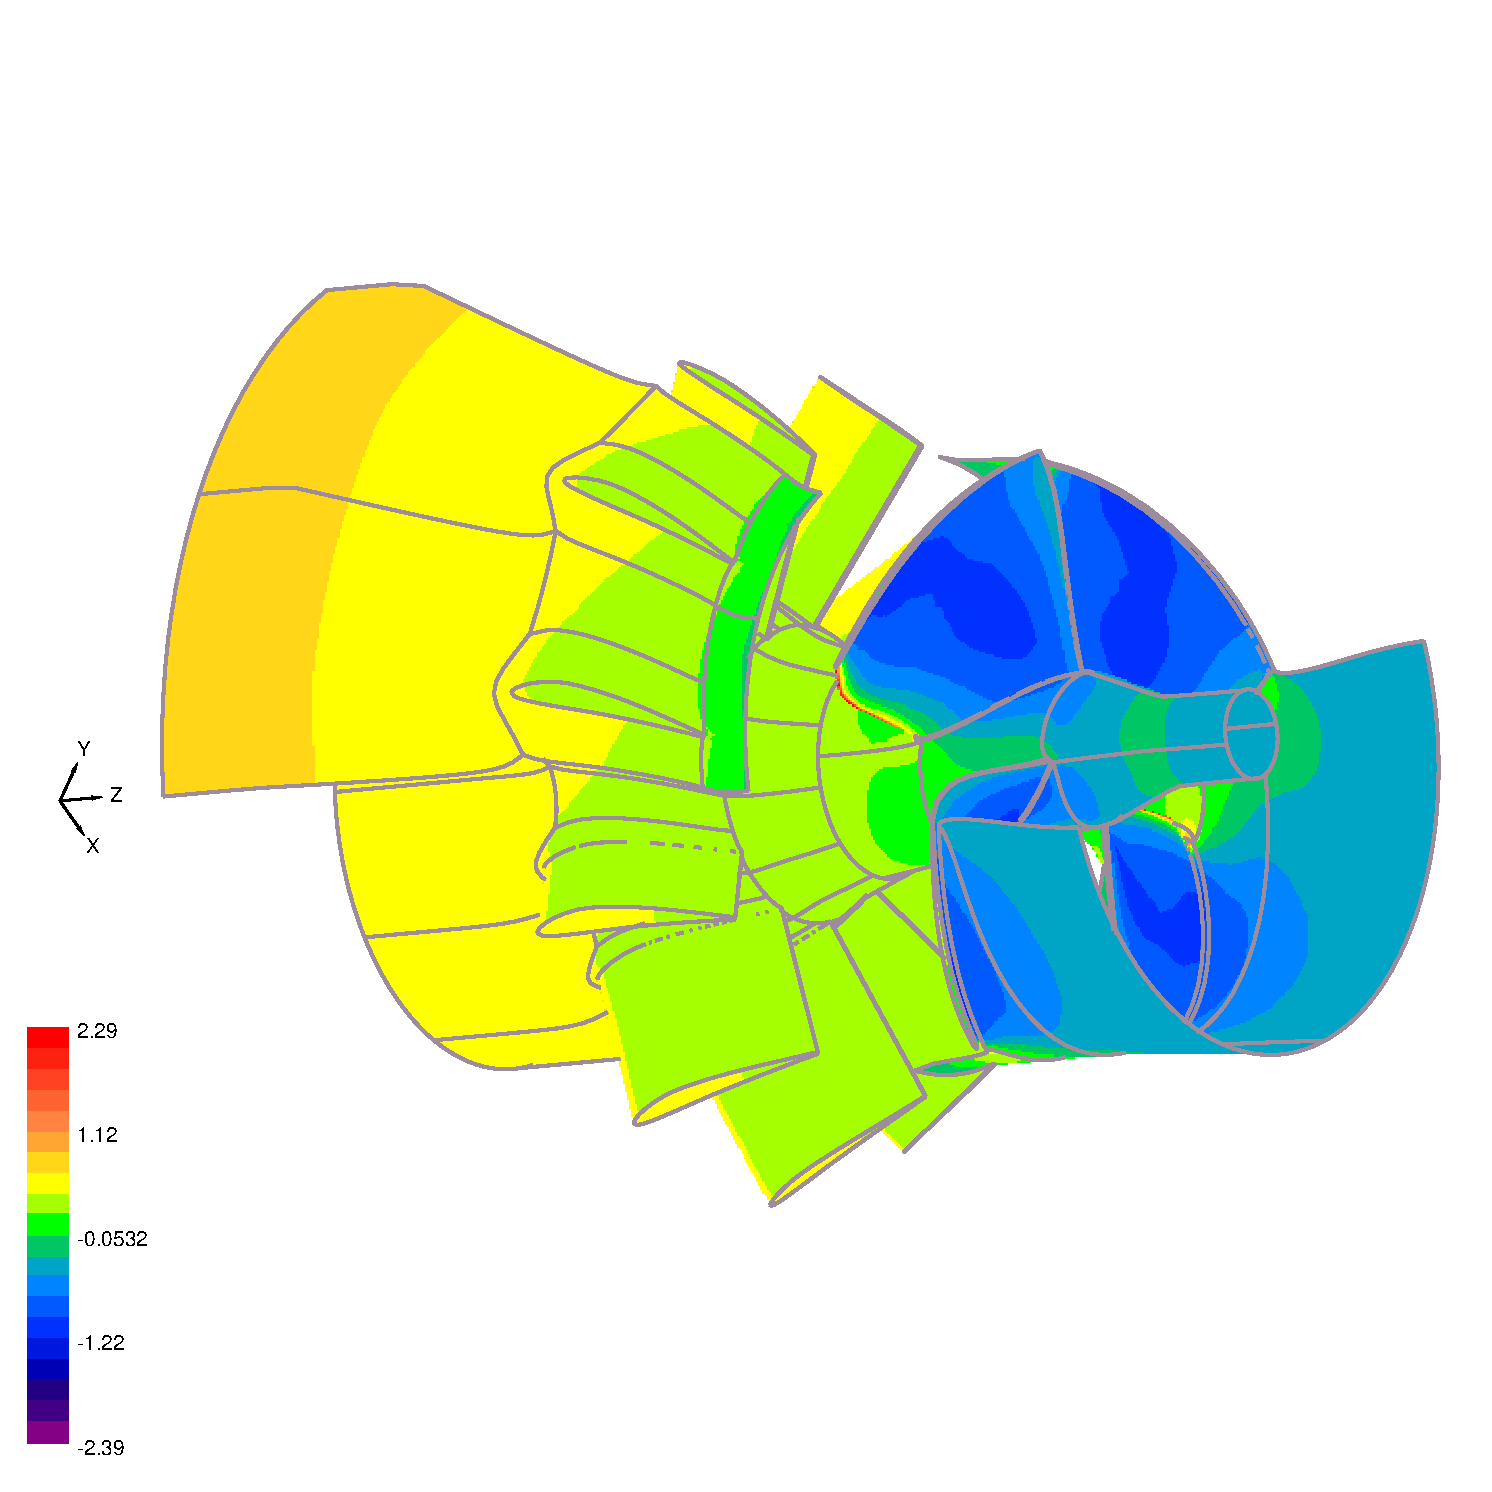
\epsfig{file=AllPress.eps,width=450\unitlength}
\newpage
{\huge Bladeload for Stator}\\ press ($\sigma$) \\
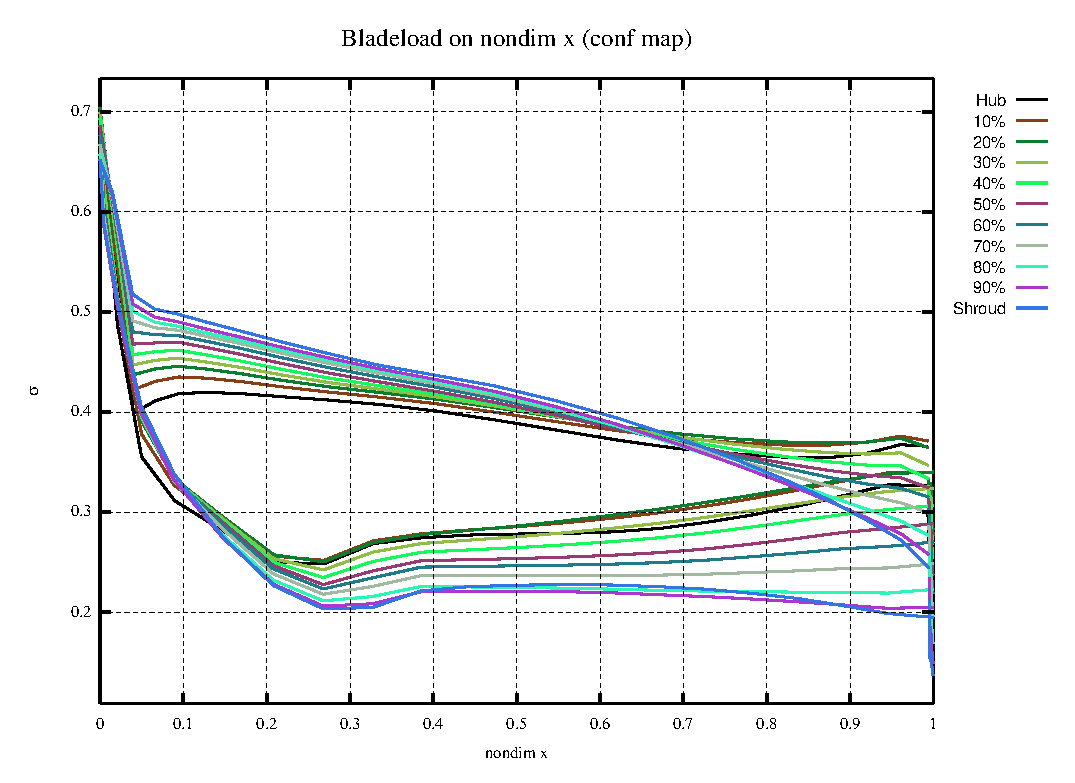
\epsfig{file=BladeLoadStator.eps,width=450\unitlength}
\newpage
{\huge Bladeload for Rotor}\\ press ($\sigma$) \\
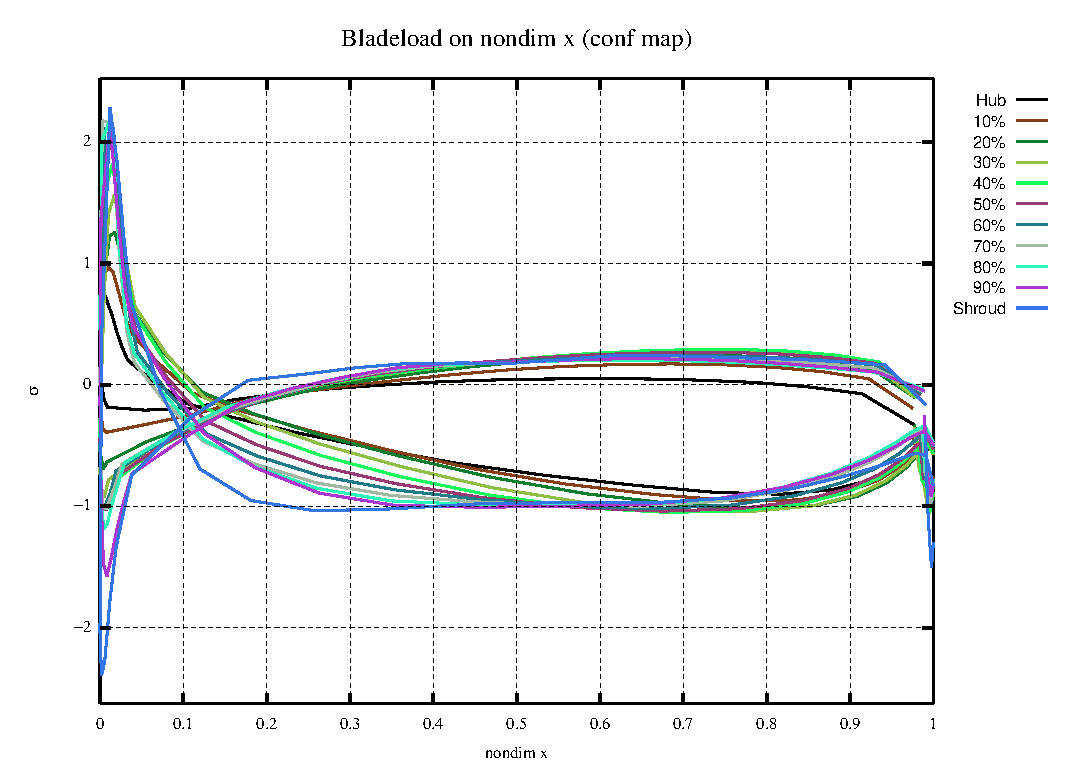
\epsfig{file=BladeLoadRotor.eps,width=450\unitlength}
\newpage
{\huge Conformal map for Stator}\\ rel. velocity ($k_c$), 0.000 span \\
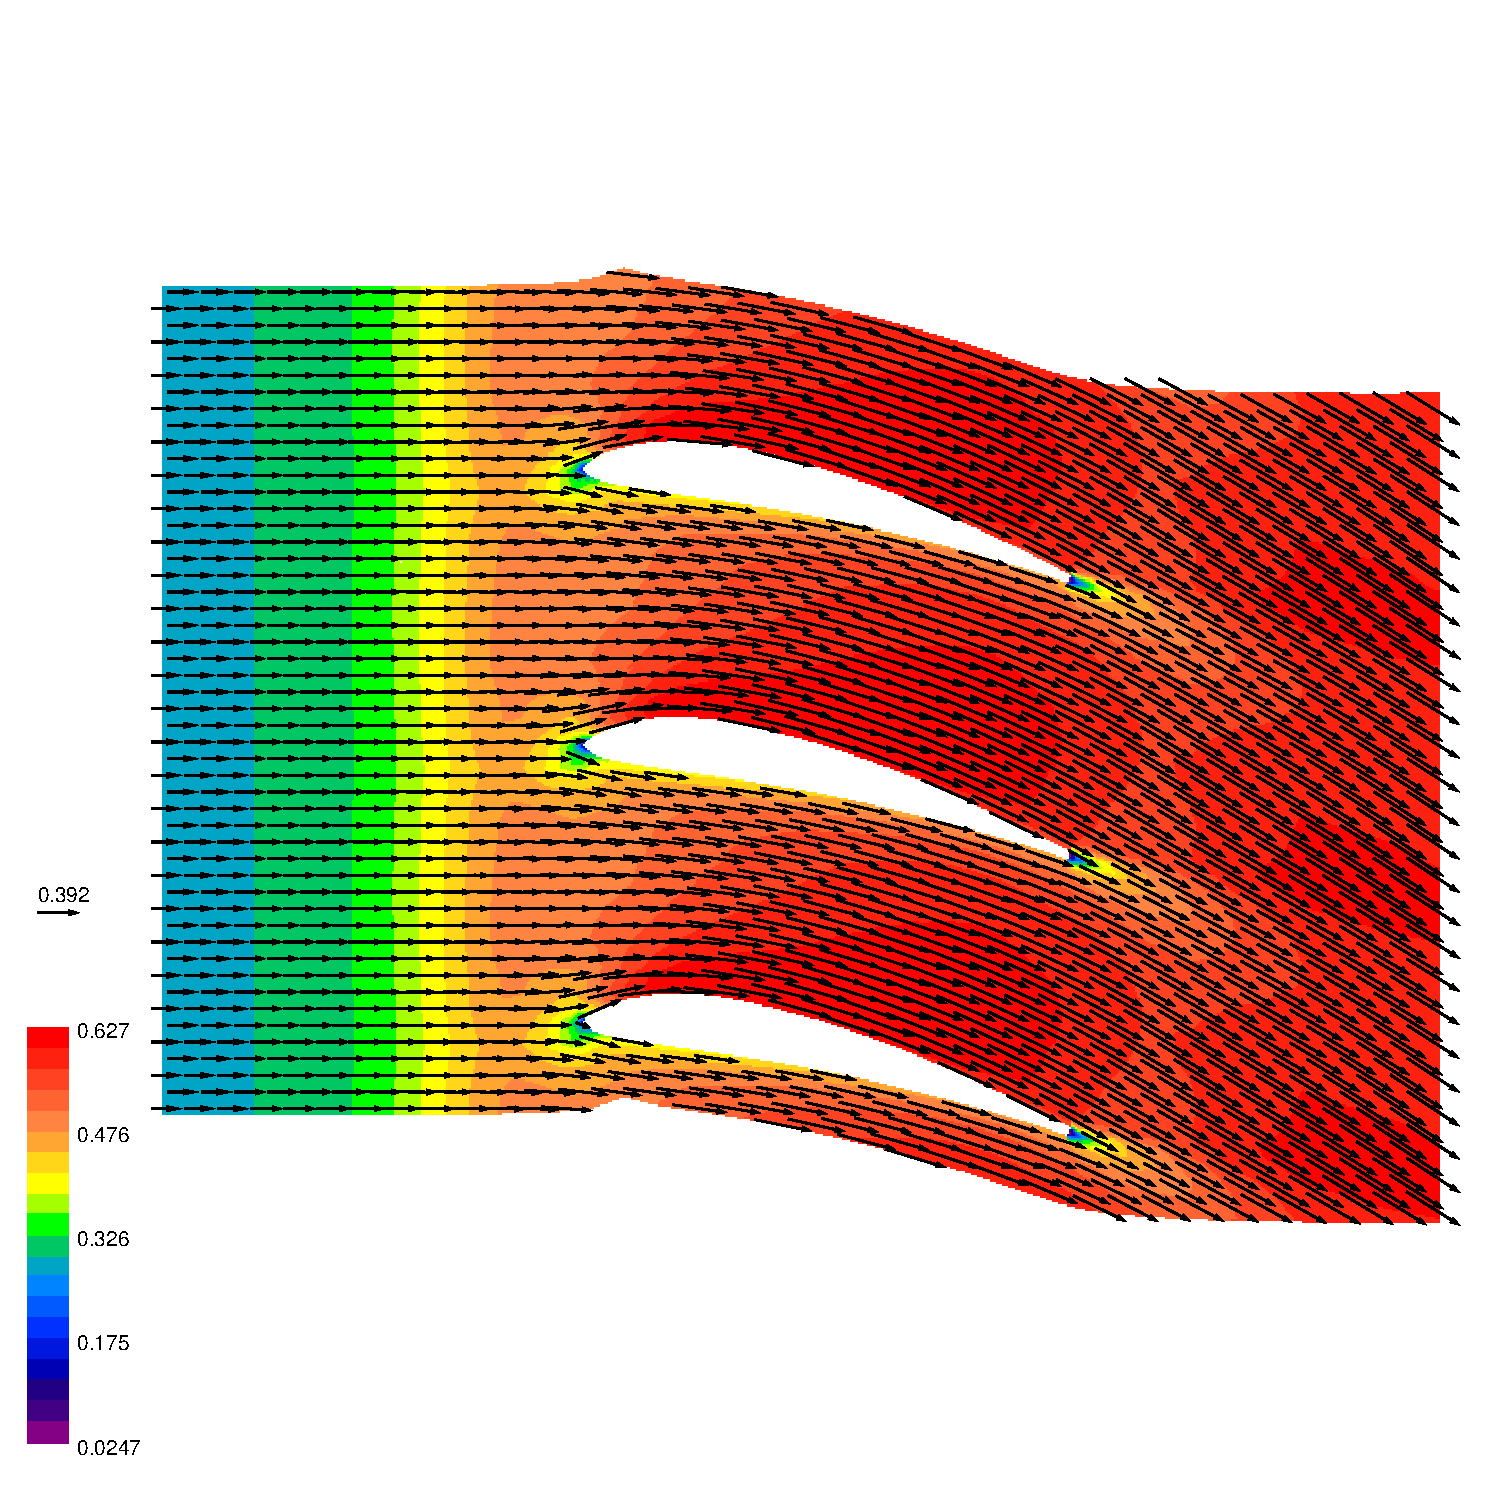
\epsfig{file=ConfMapStator0.eps,width=450\unitlength}
\newpage
{\huge Conformal map for Stator}\\ rel. velocity ($k_c$), 0.500 span \\
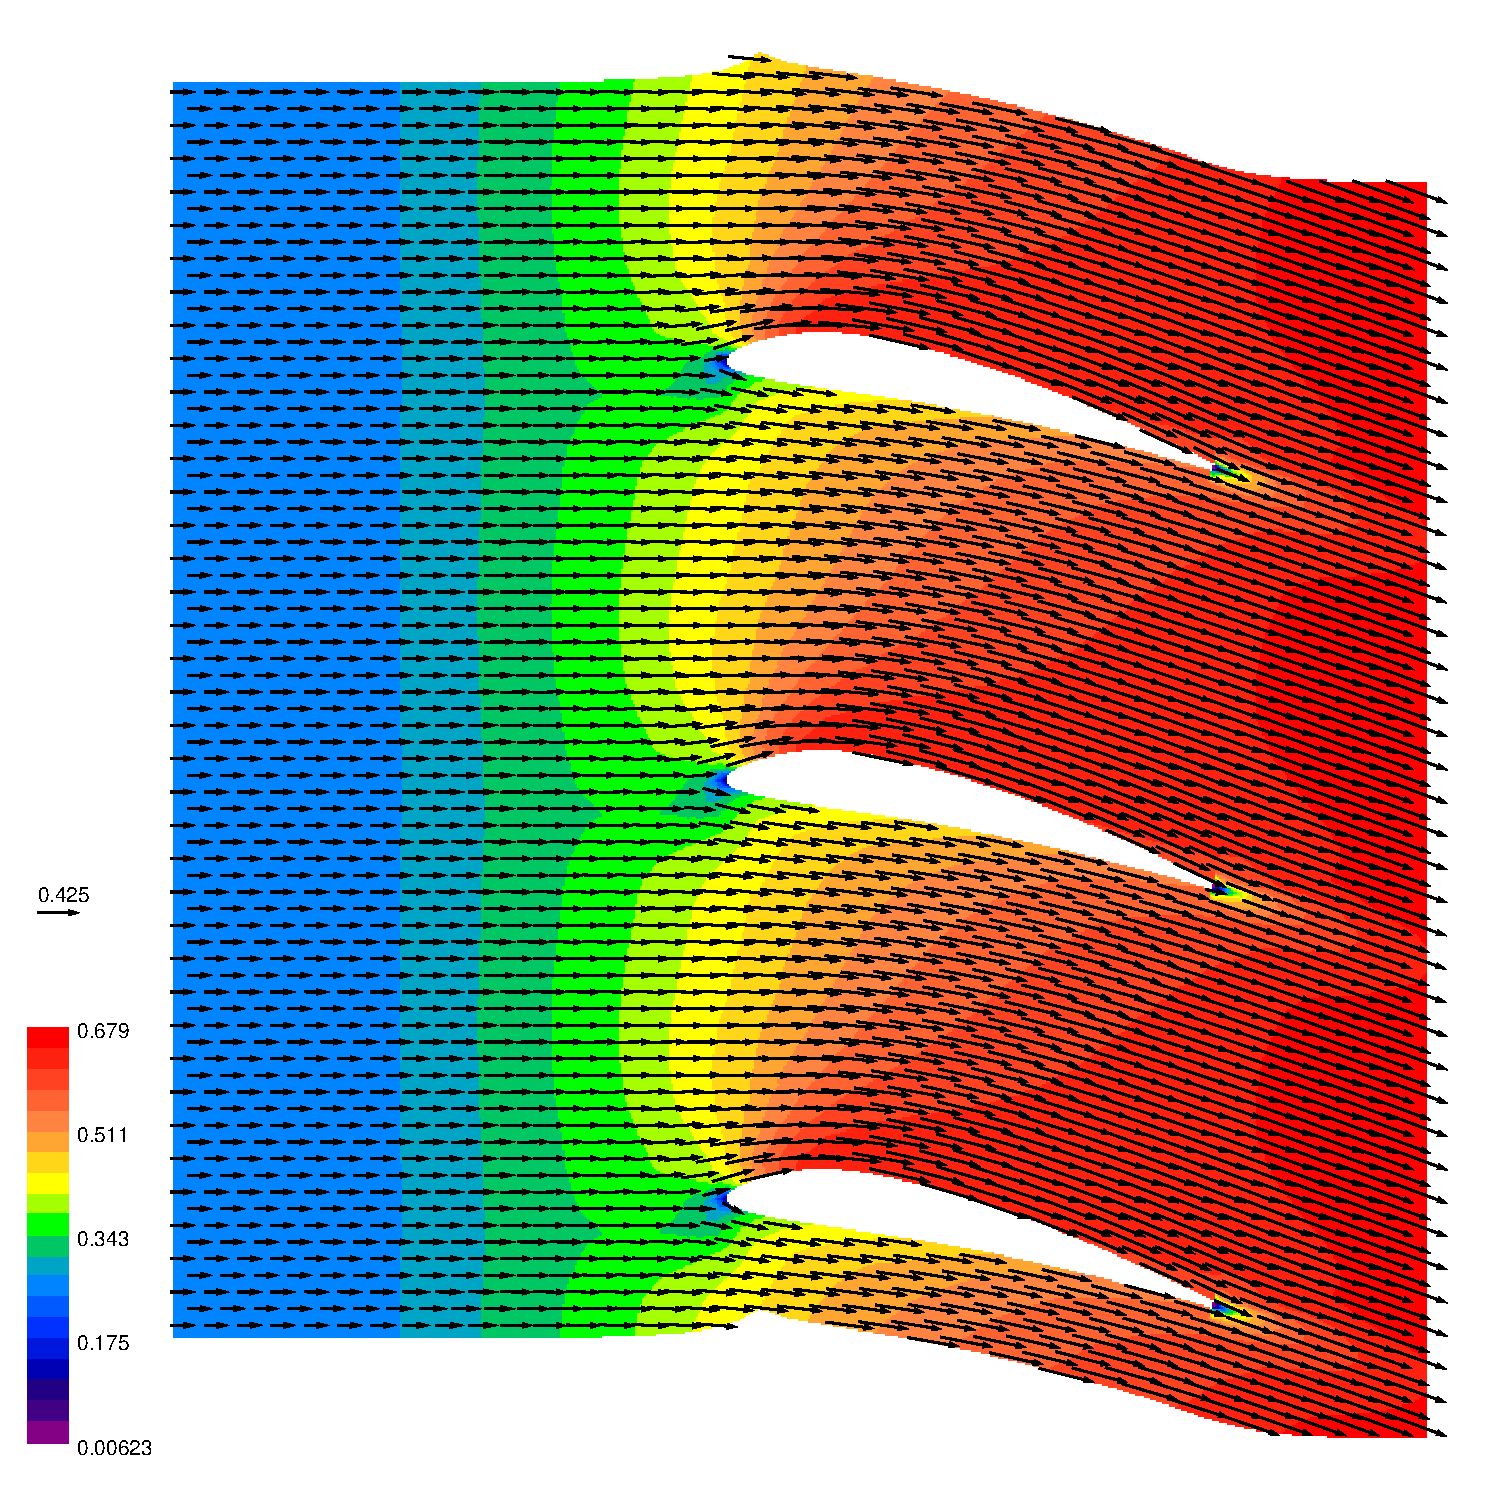
\epsfig{file=ConfMapStator1.eps,width=450\unitlength}
\newpage
{\huge Conformal map for Stator}\\ rel. velocity ($k_c$), 1.000 span \\
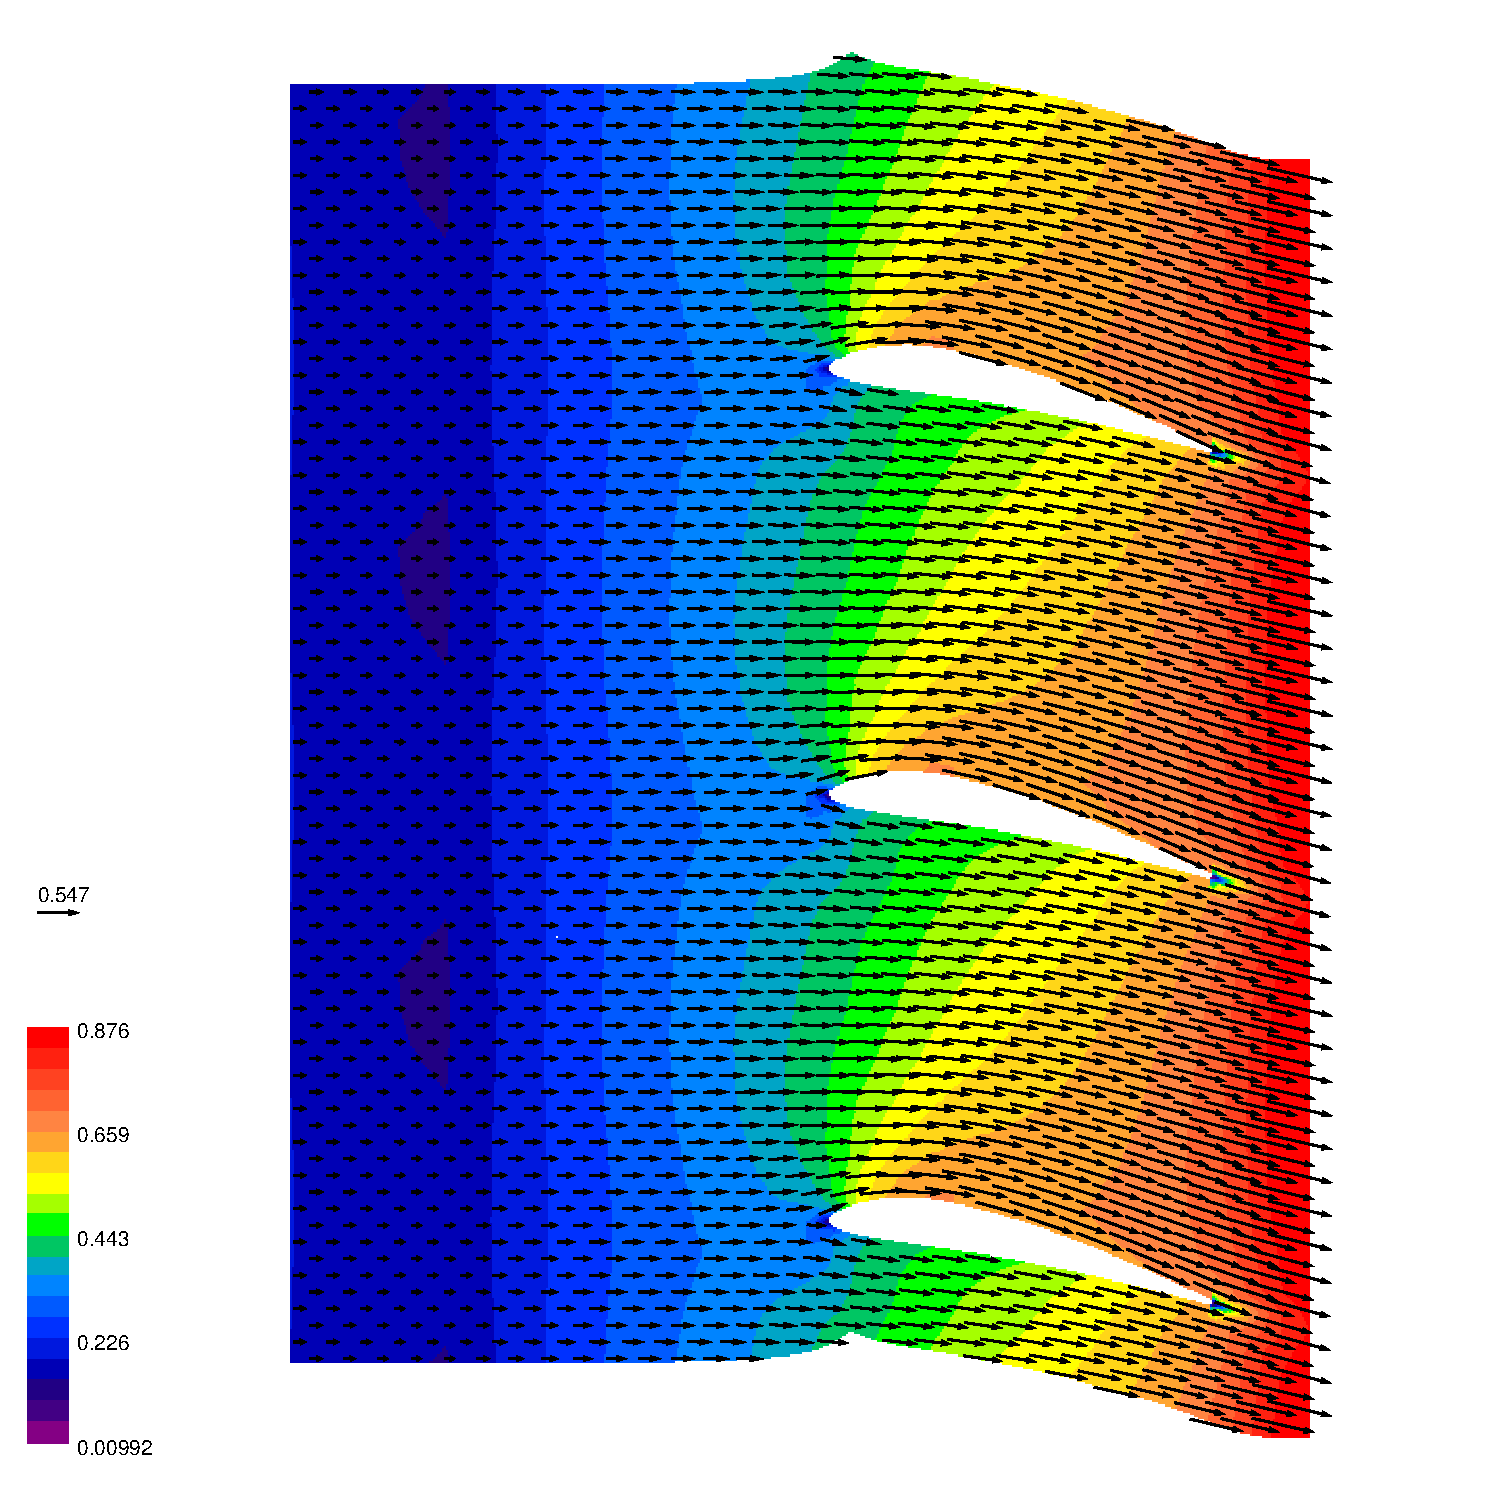
\epsfig{file=ConfMapStator2.eps,width=450\unitlength}
\newpage
{\huge Conformal map for Rotor}\\ rel. velocity ($k_c$), 0.000 span \\
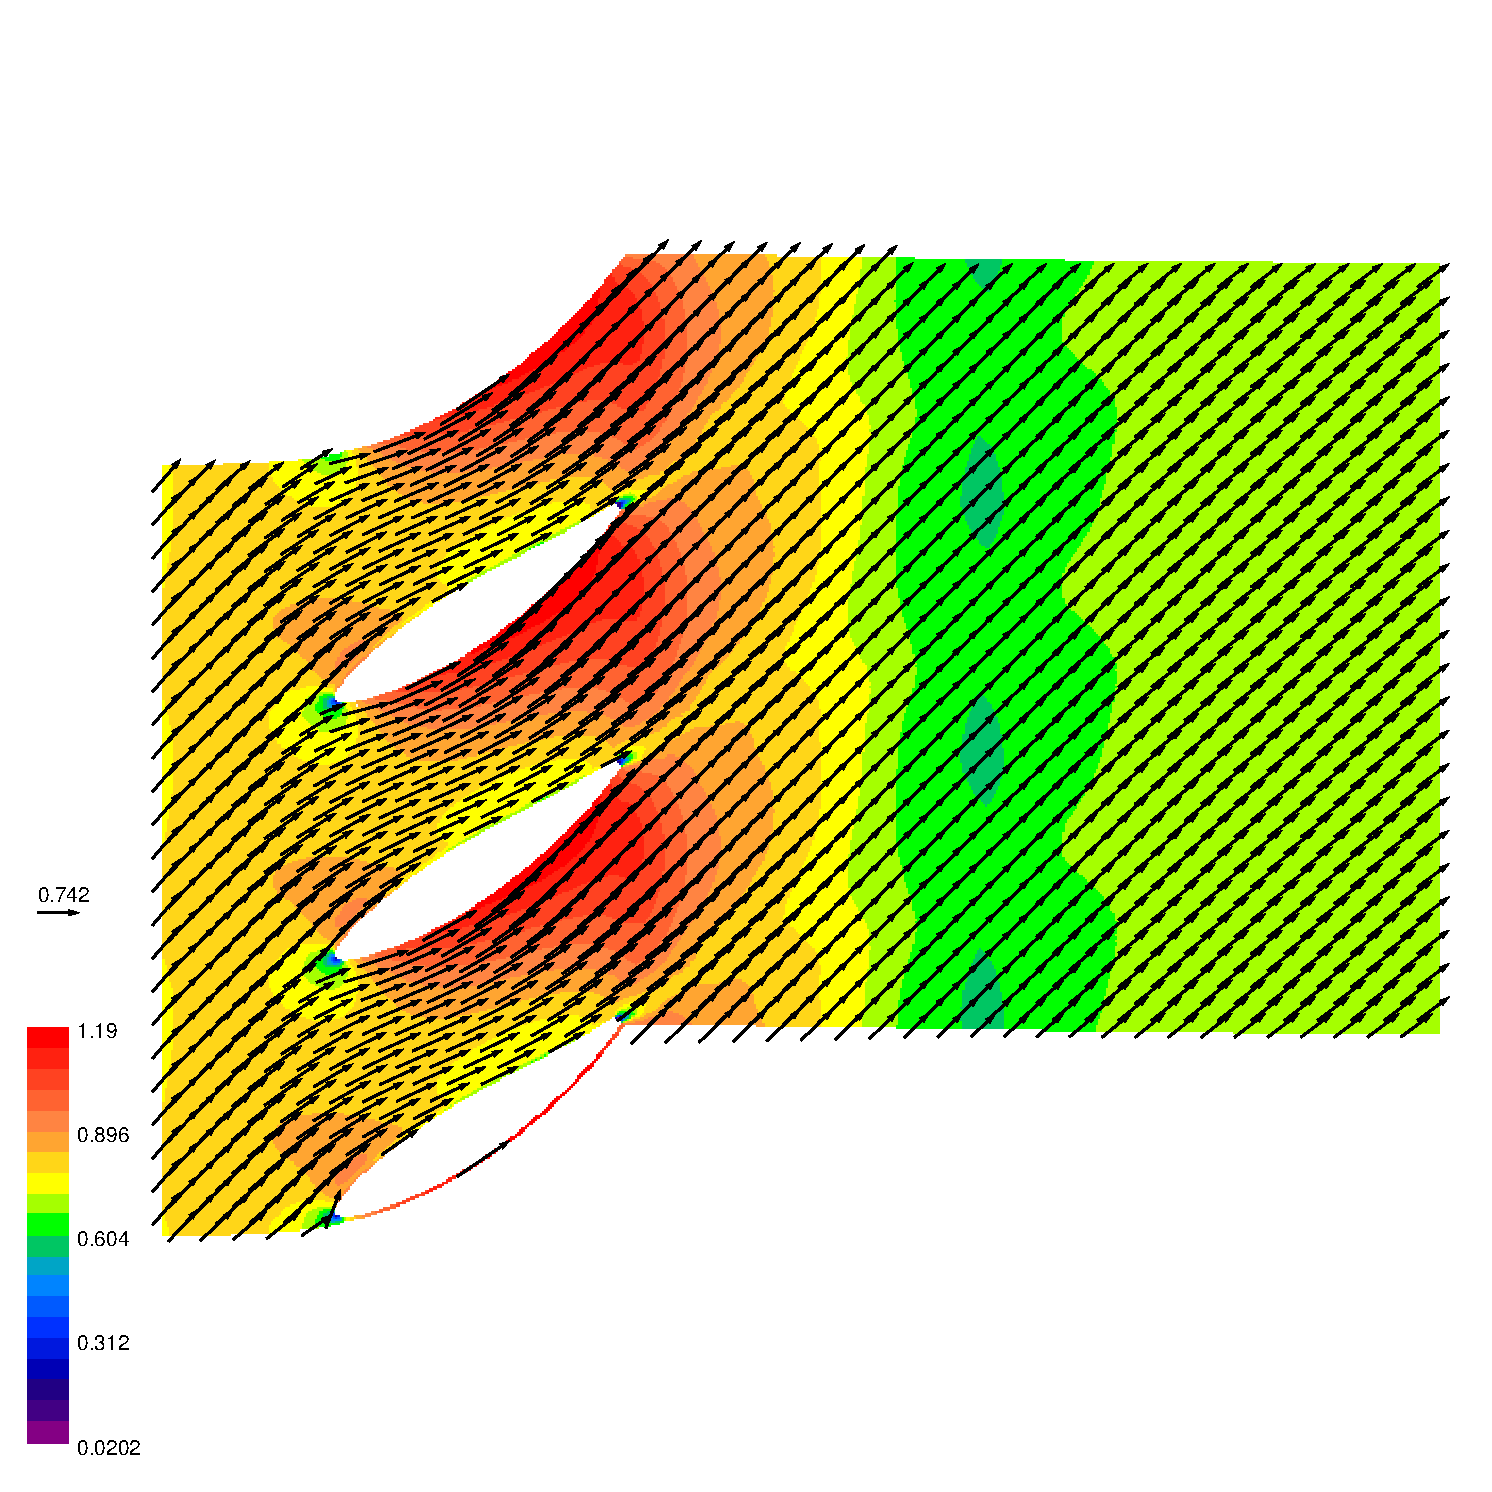
\epsfig{file=ConfMapRotor0.eps,width=450\unitlength}
\newpage
{\huge Conformal map for Rotor}\\ rel. velocity ($k_c$), 0.500 span \\
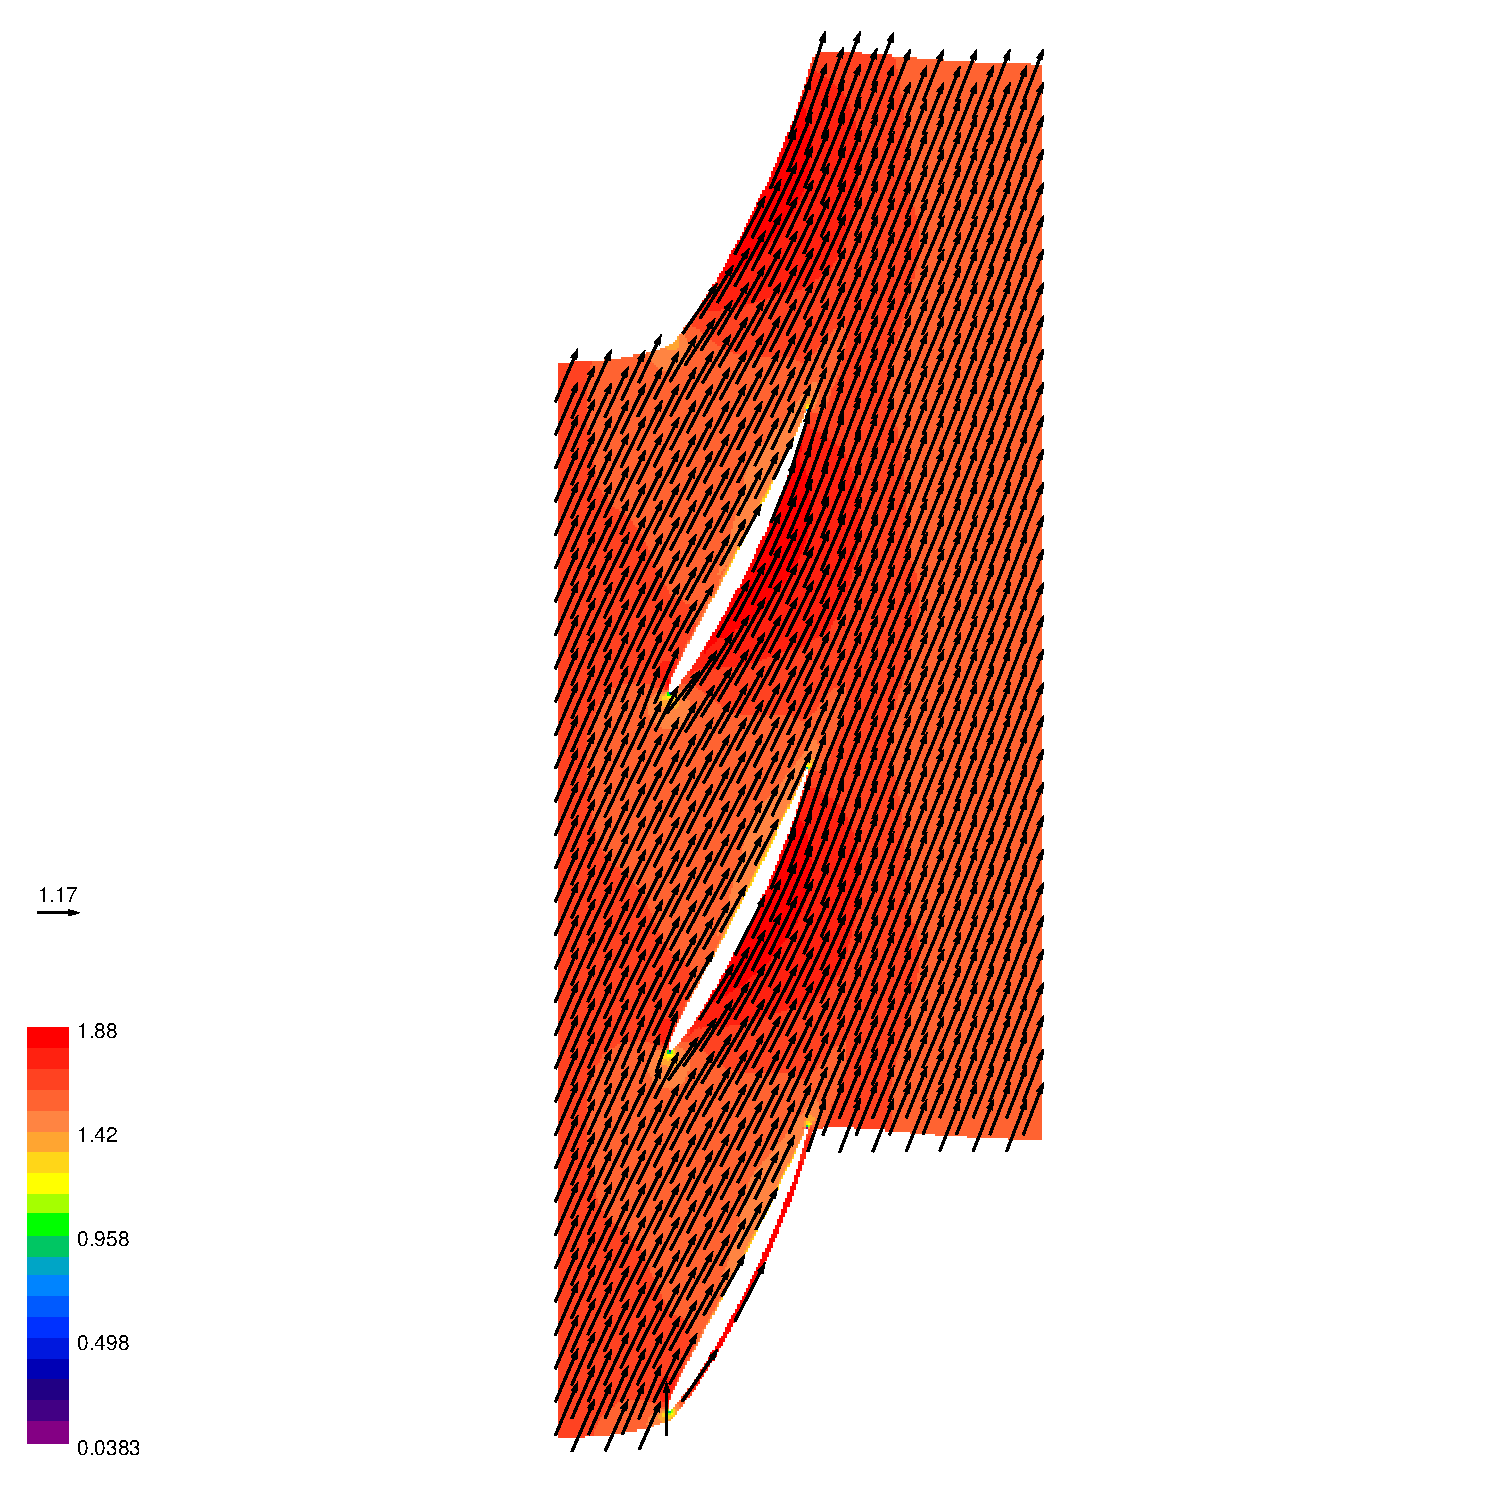
\epsfig{file=ConfMapRotor1.eps,width=450\unitlength}
\newpage
{\huge Conformal map for Rotor}\\ rel. velocity ($k_c$), 0.750 span \\
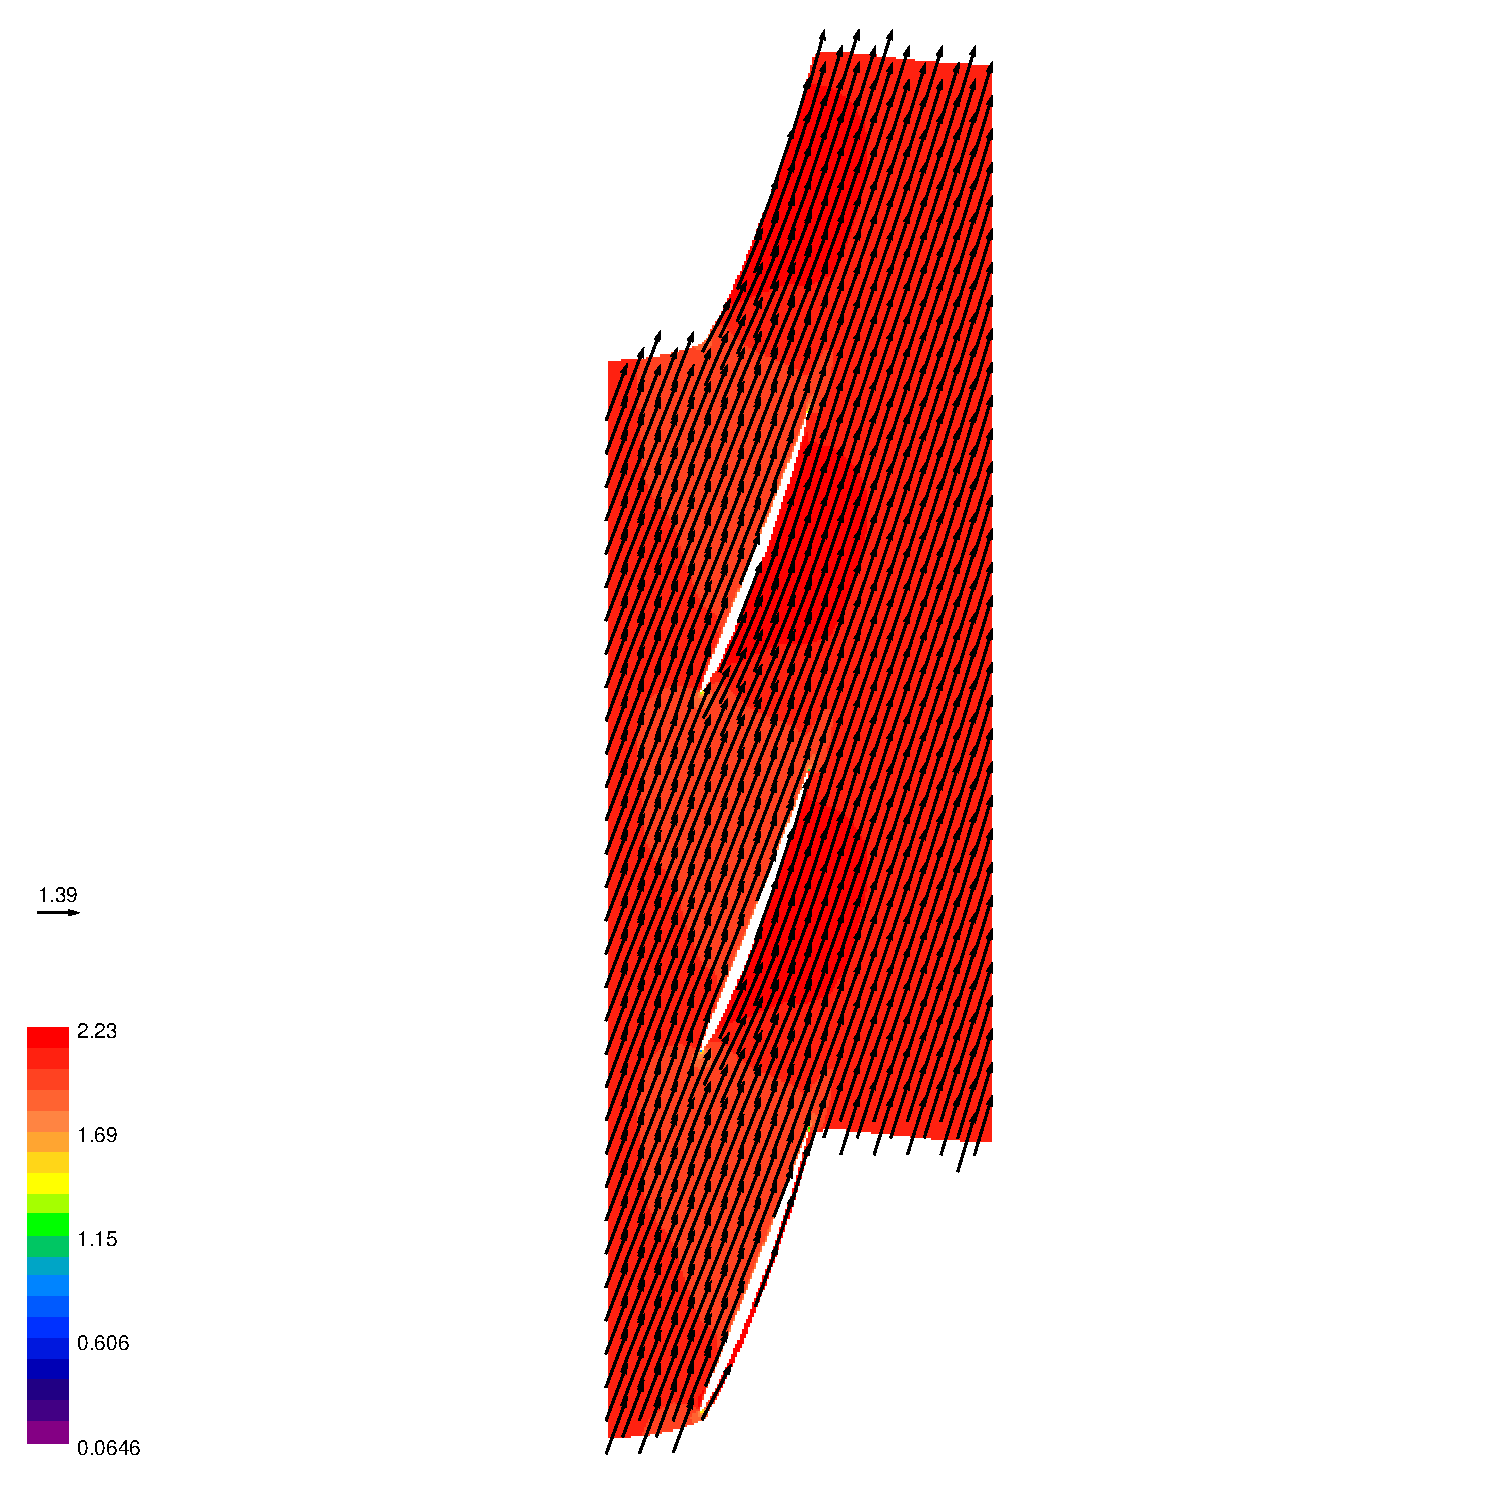
\epsfig{file=ConfMapRotor2.eps,width=450\unitlength}
\newpage
{\huge Conformal map for Rotor}\\ rel. velocity ($k_c$), 1.000 span \\
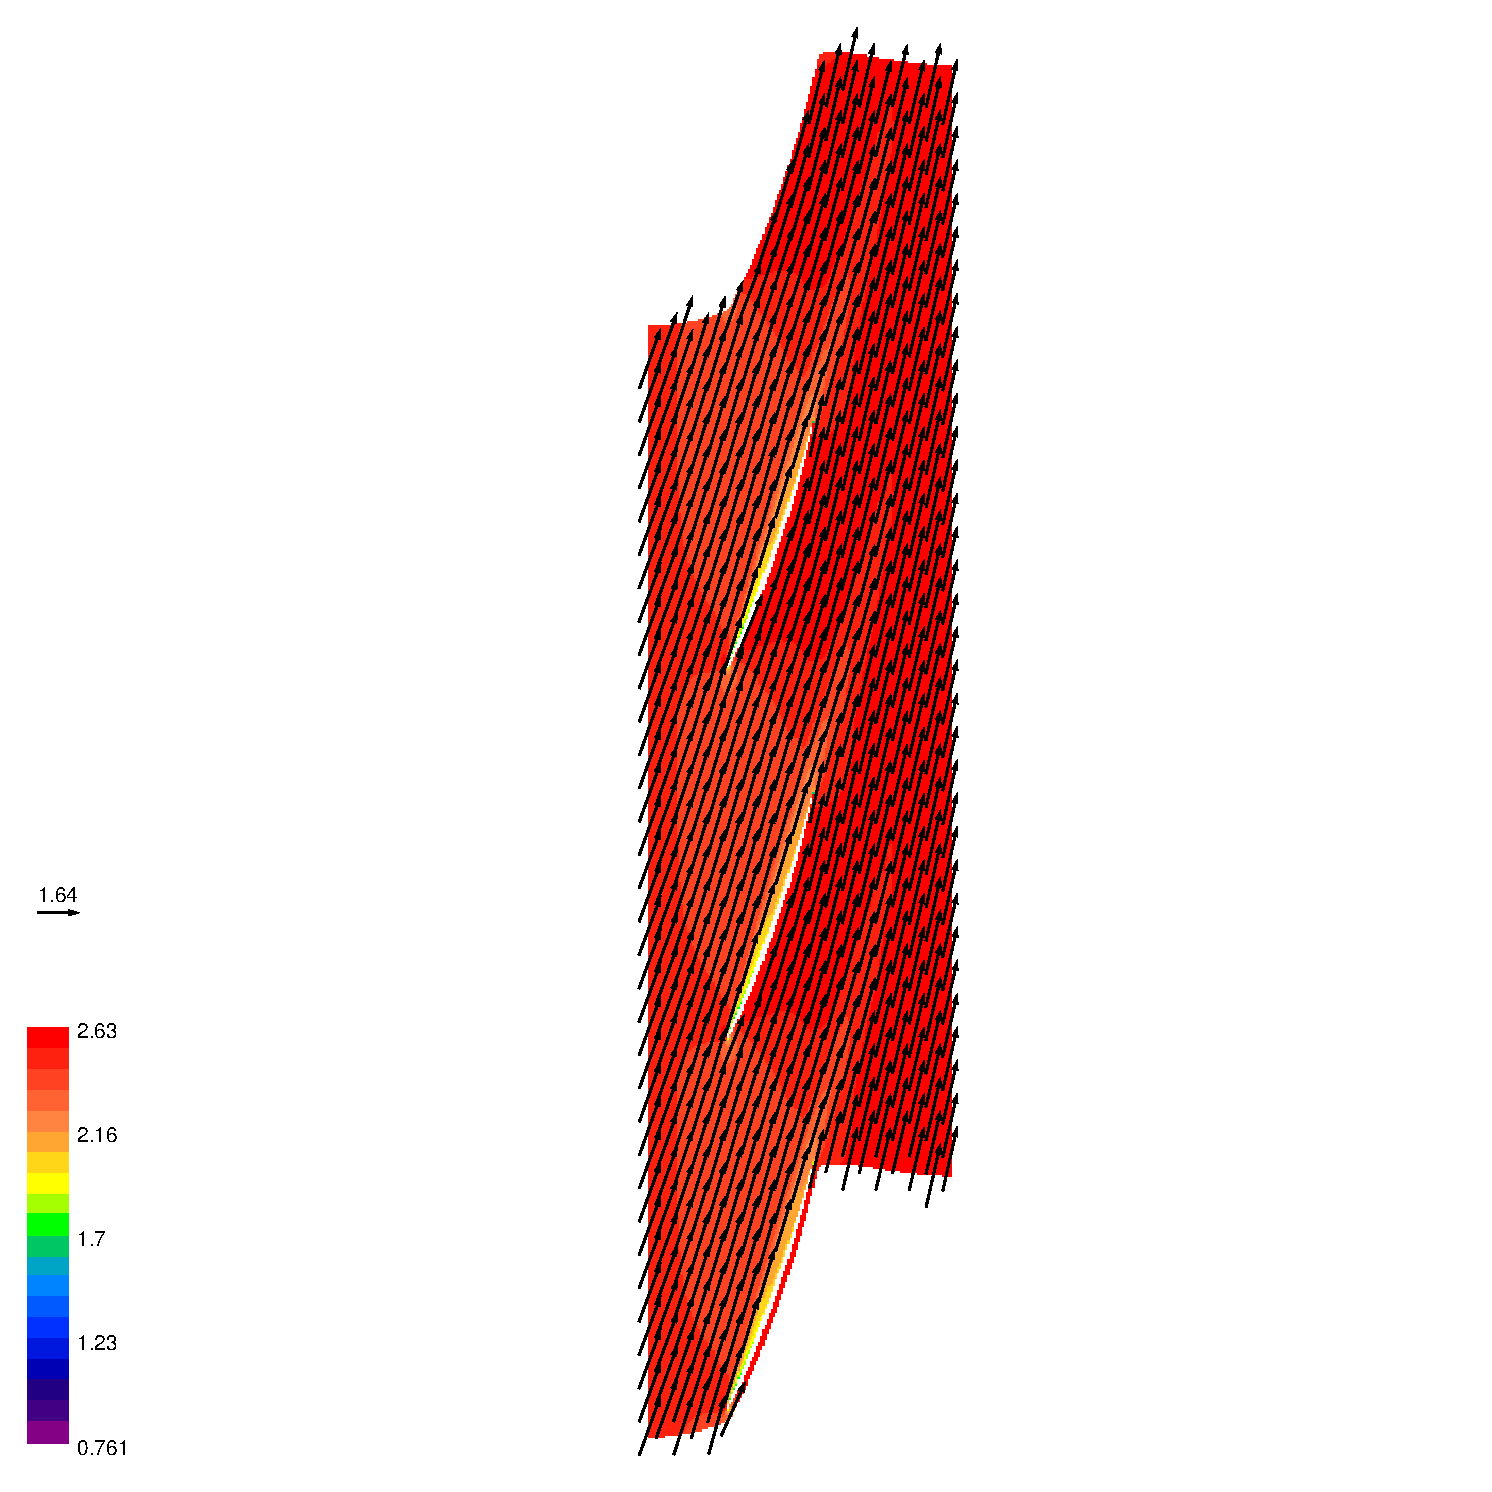
\epsfig{file=ConfMapRotor3.eps,width=450\unitlength}
\newpage
{\huge Blade of Stator, side 1}\\ press ($\sigma$) and rel. velocity ($k_c$)\\
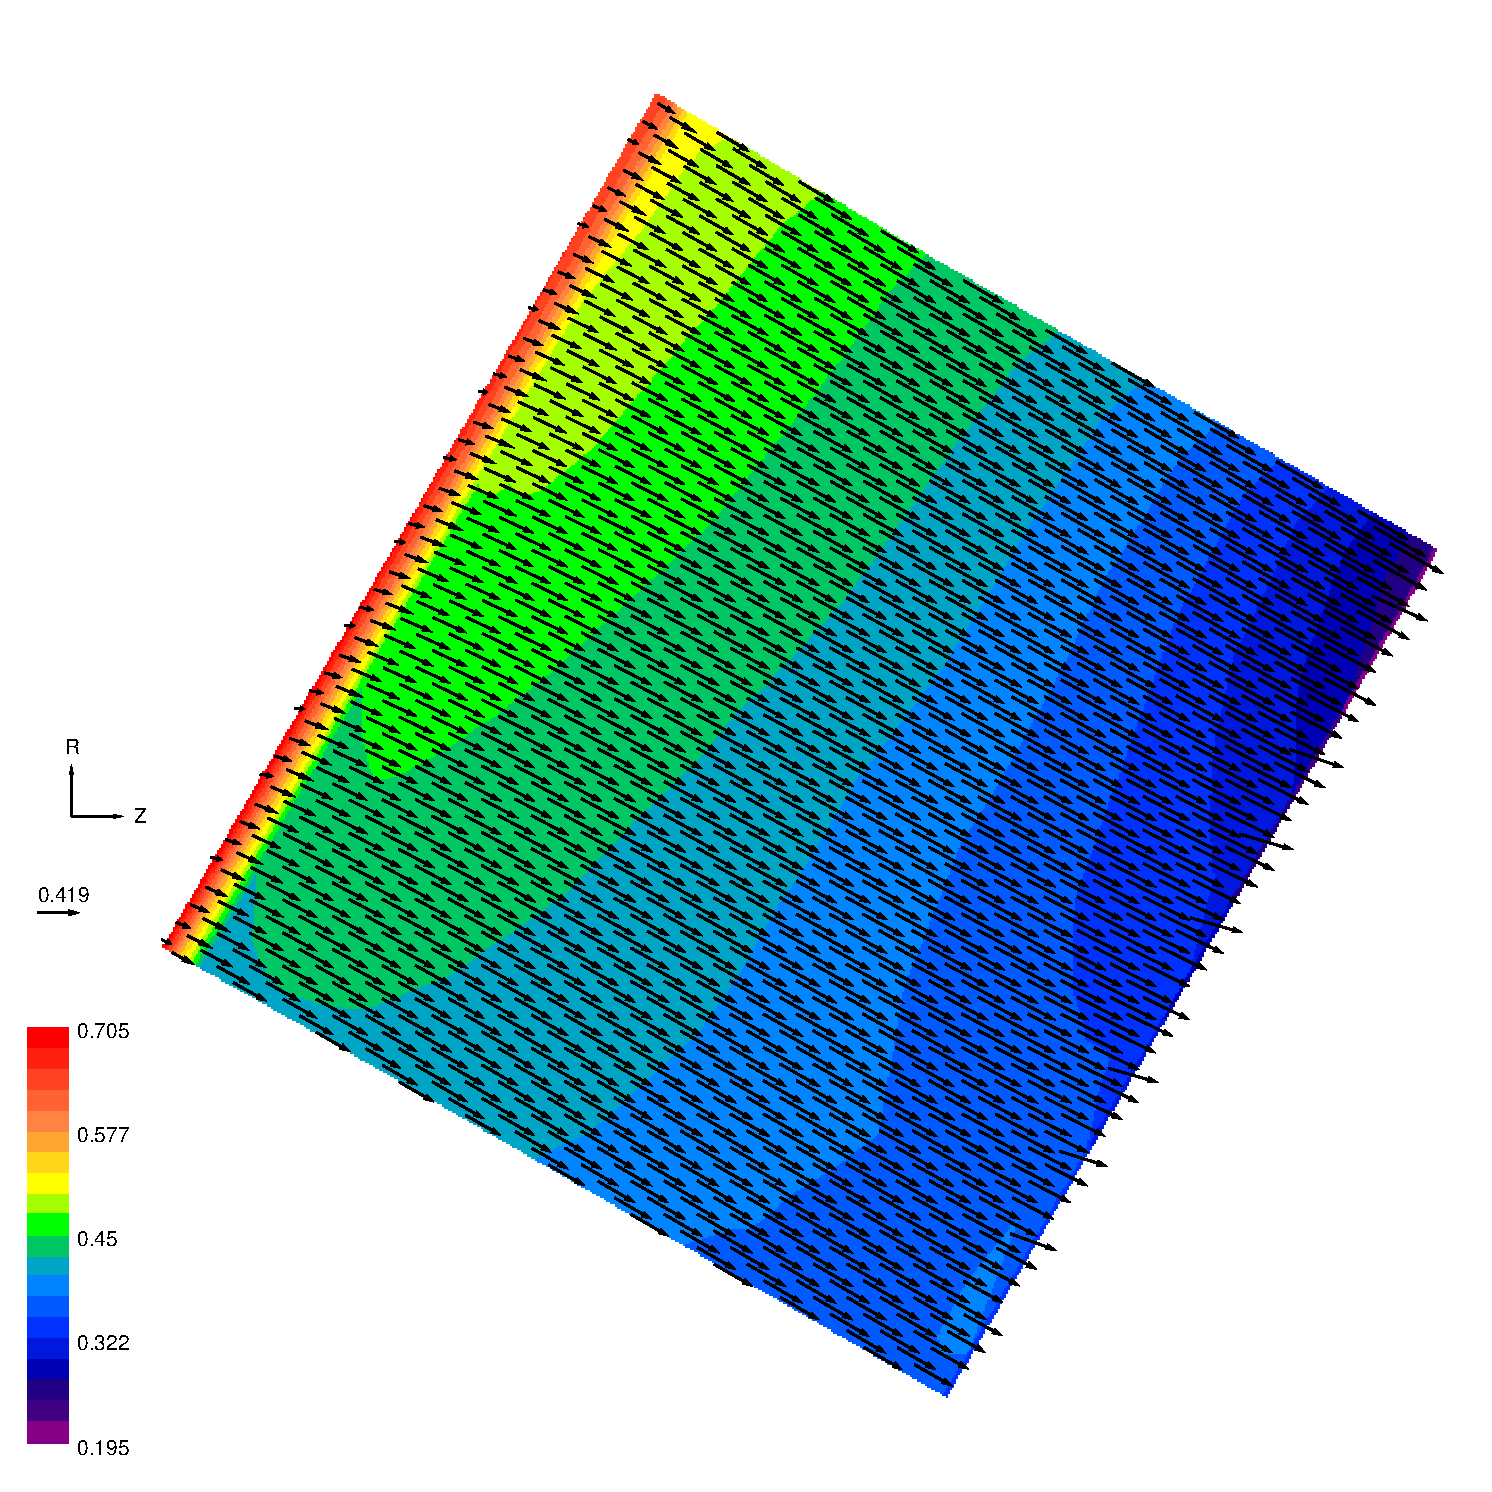
\epsfig{file=BladeZylStator1.eps,width=450\unitlength}
\newpage
{\huge Blade of Stator, side 2}\\ press ($\sigma$)  and rel. velocity ($k_c$)\\
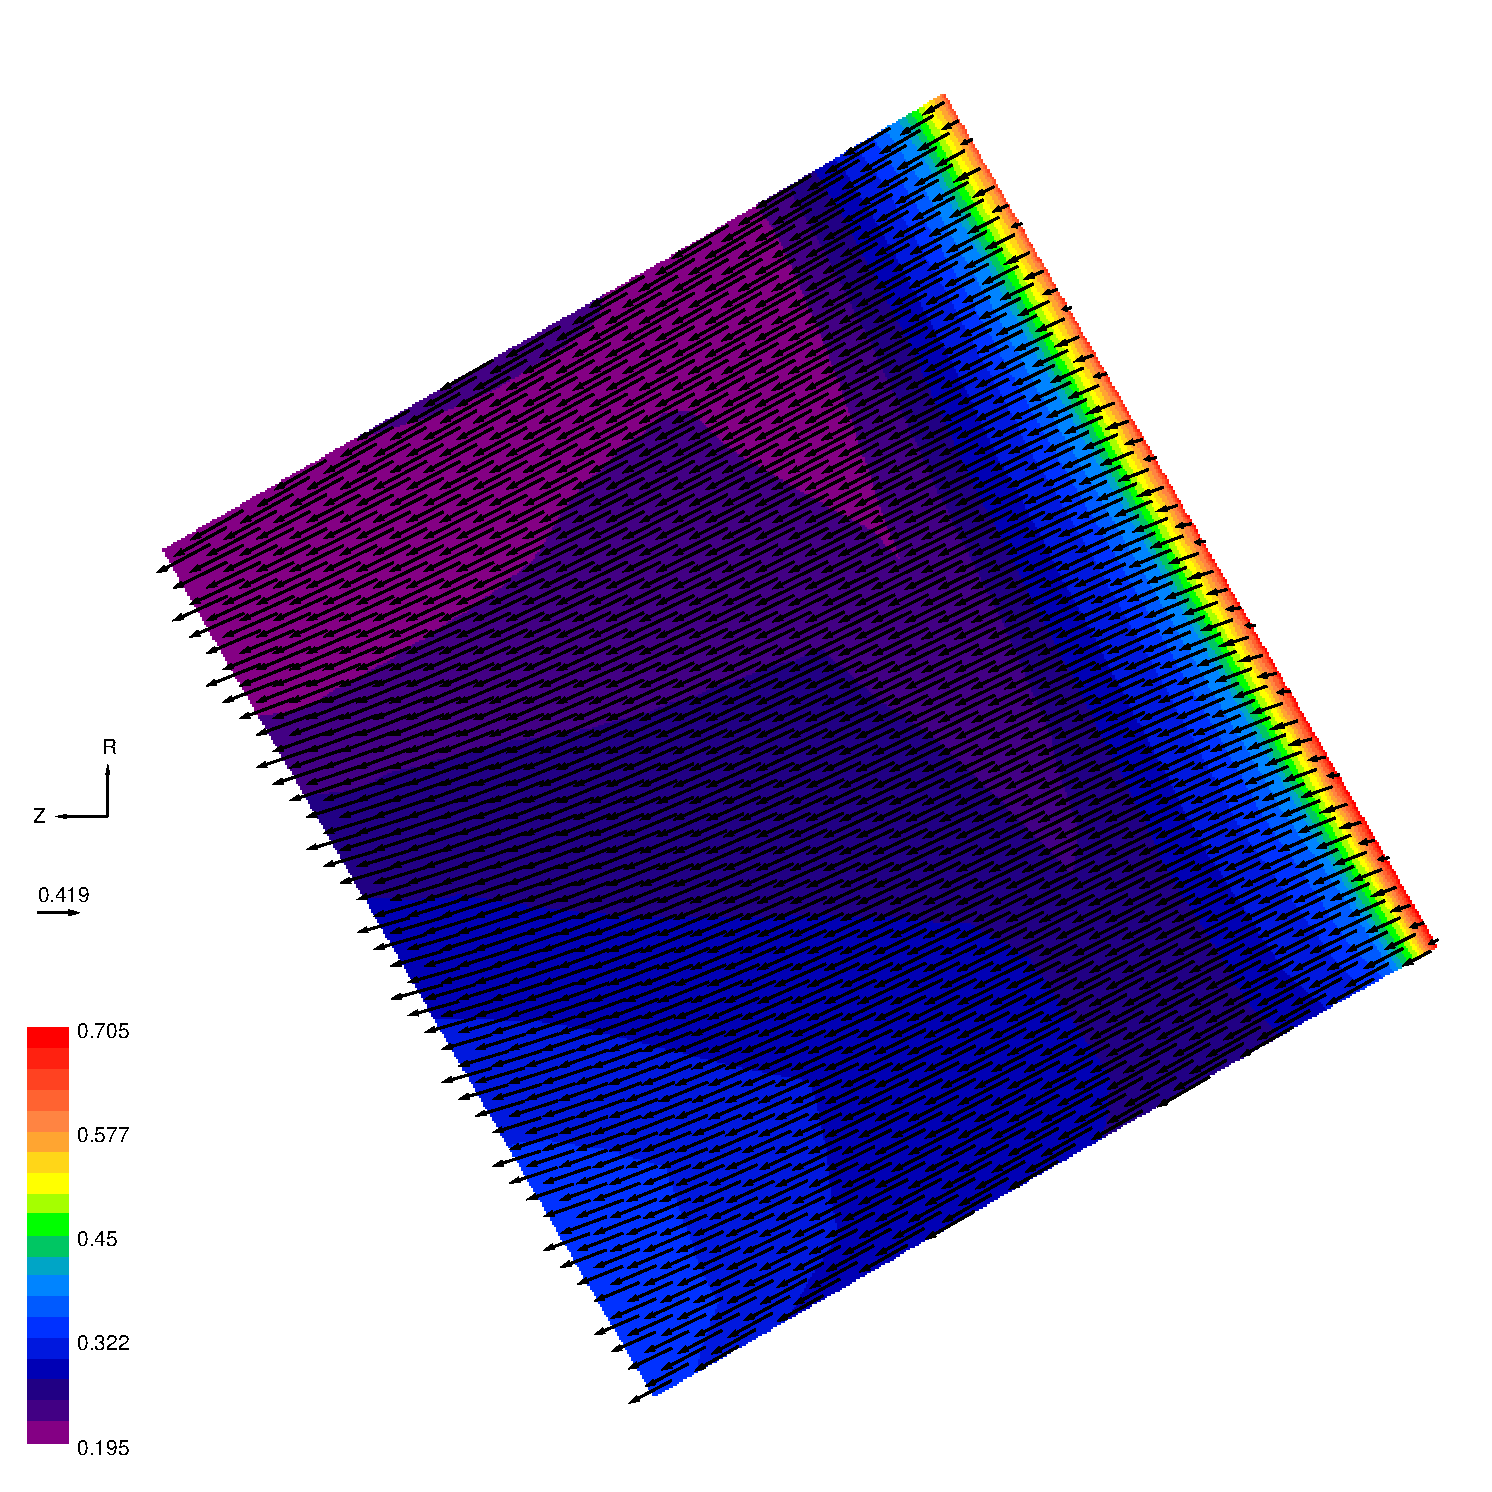
\epsfig{file=BladeZylStator2.eps,width=450\unitlength}
\newpage
{\huge Blade of Rotor, side 1}\\ press ($\sigma$) and rel. velocity ($k_c$)\\
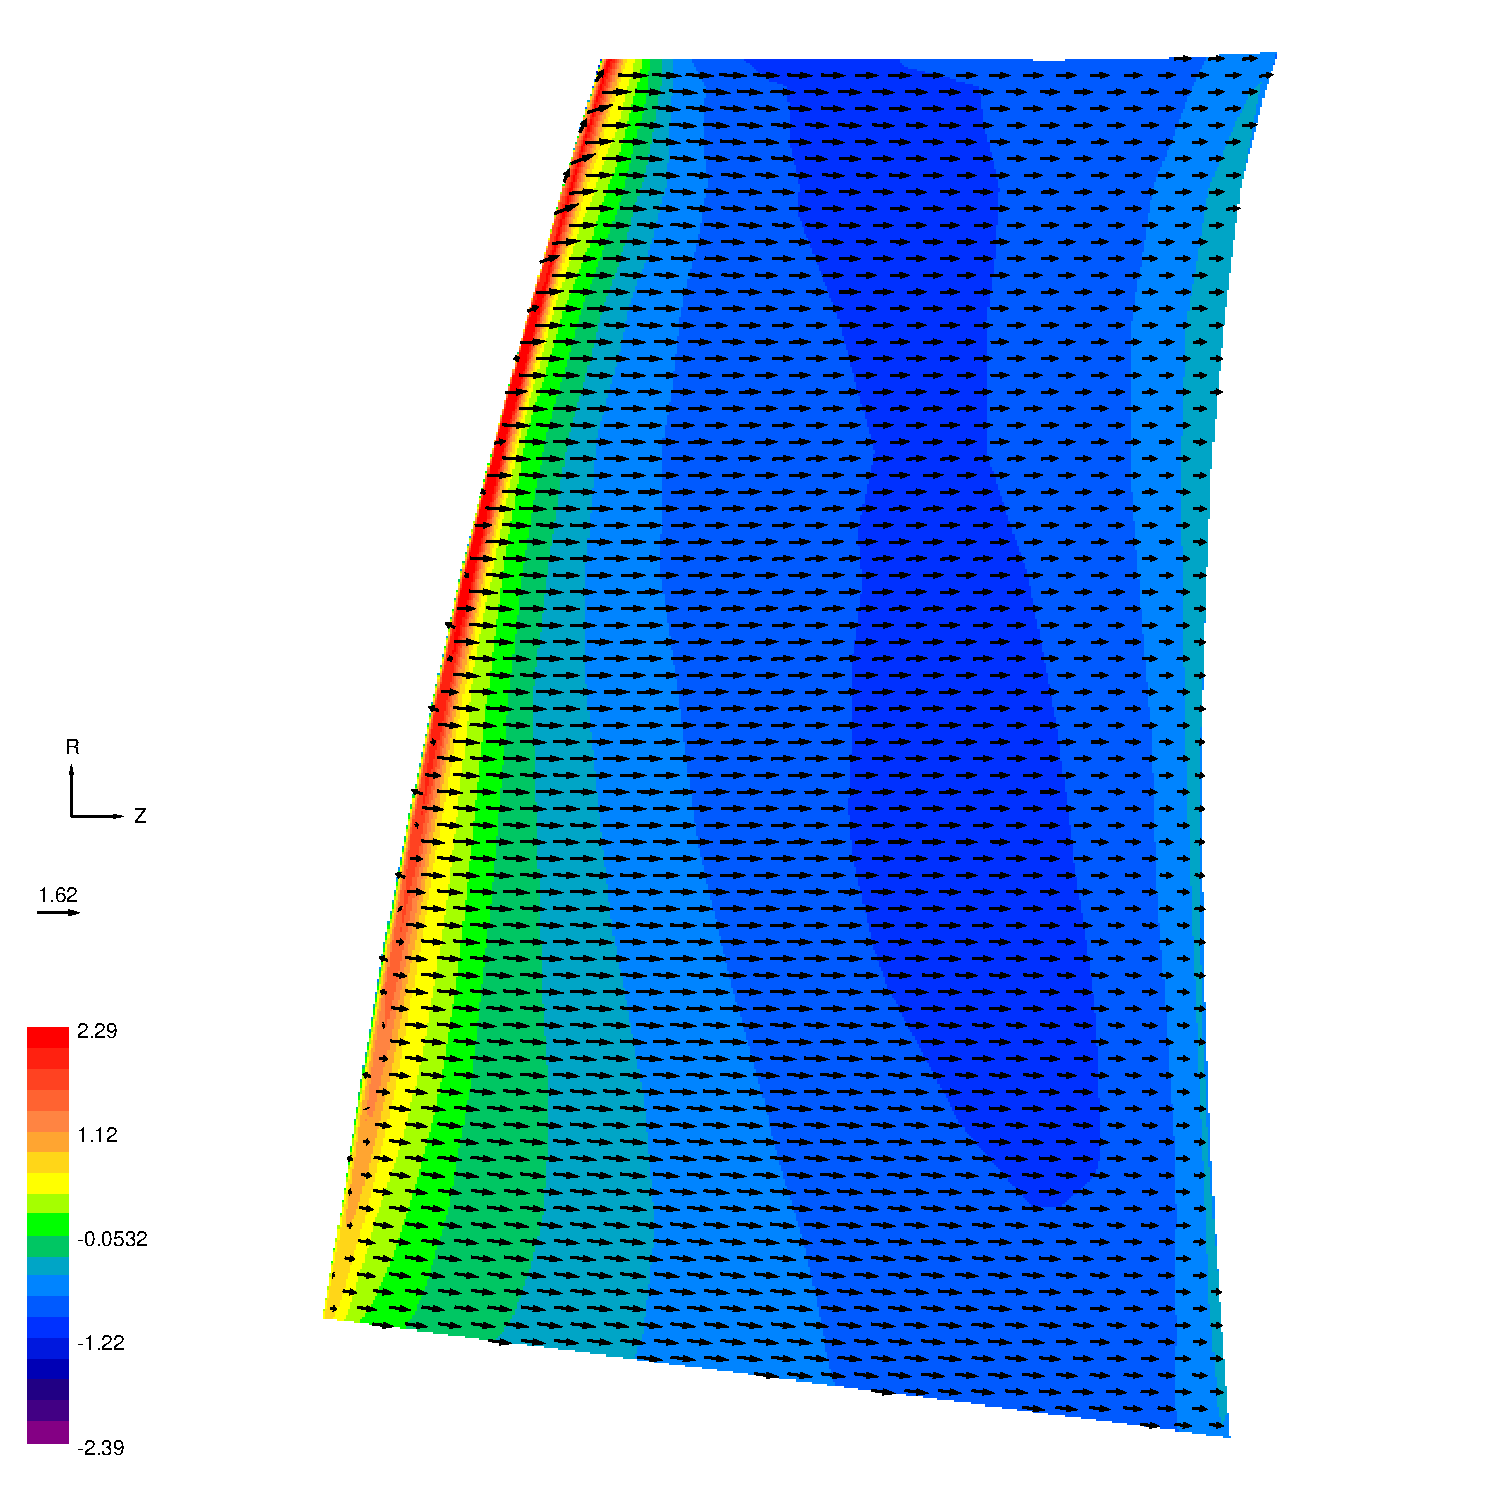
\epsfig{file=BladeZylRotor1.eps,width=450\unitlength}
\newpage
{\huge Blade of Rotor, side 2}\\ press ($\sigma$)  and rel. velocity ($k_c$)\\
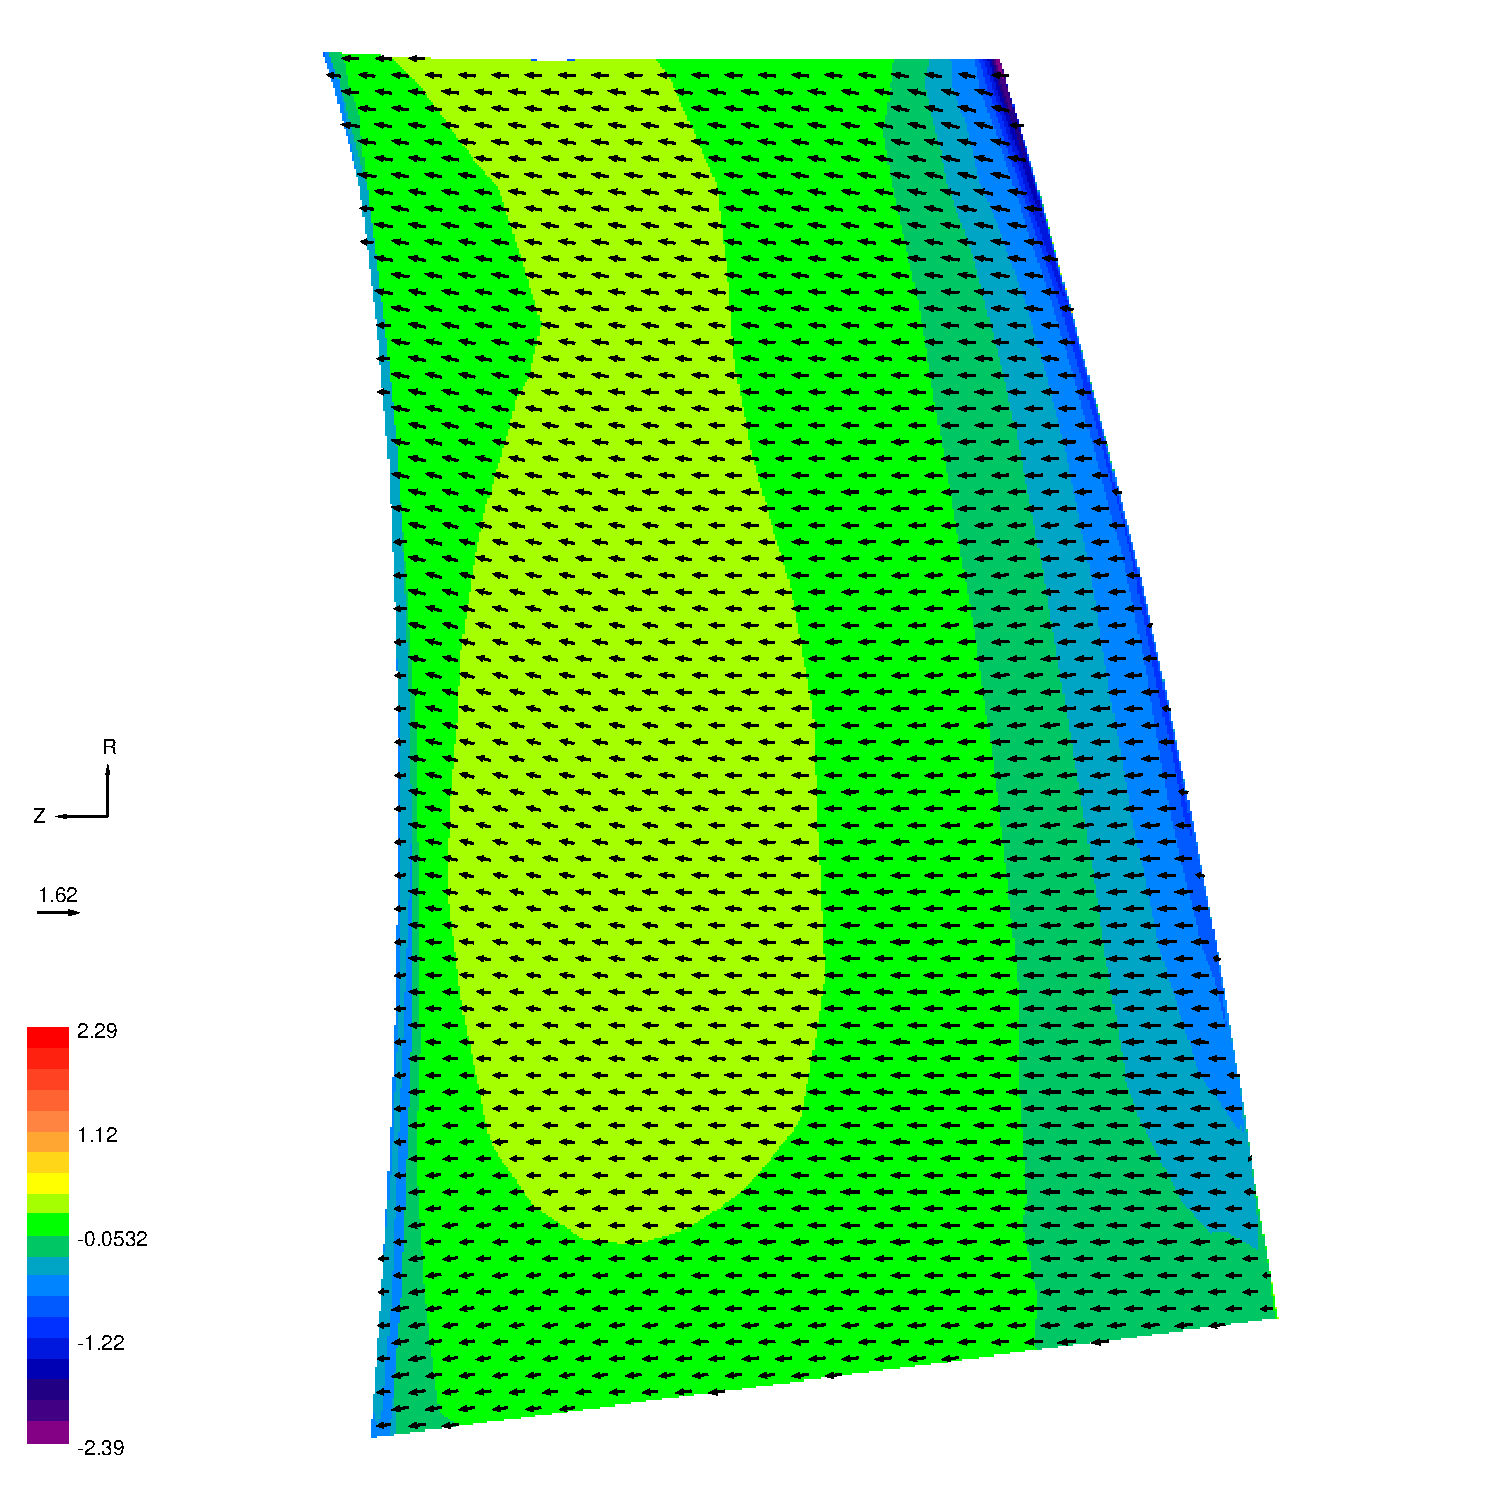
\epsfig{file=BladeZylRotor2.eps,width=450\unitlength}

\end{document}

